\documentclass{article}

% Language setting
\usepackage[spanish,es-nodecimaldot]{babel}

\usepackage[letterpaper,top=2cm,bottom=3.5cm,left=2.5cm,right=2.5cm,marginparwidth=1.75cm]{geometry}

% Useful packages
\usepackage{amsmath}
\usepackage{tabularx}
\usepackage{graphicx}
\usepackage[colorlinks=true, allcolors=blue]{hyperref}
\usepackage{amssymb} 
\usepackage{fancyhdr}
\usepackage{multicol}
\usepackage{booktabs}
\usepackage{float}
\pagestyle{fancy} 

\fancyhf{} % Limpiar encabezado y pie de página por defecto
\setlength{\headheight}{70pt} % Ajuste del tamaño del encabezado

% Definición del encabezado institucional
\fancyhead[C]{%
    \begin{minipage}[c]{2.0cm}
        \centering
        
\includegraphics[width=2.0cm]{imagenes/uta.png}
    \end{minipage}%
    \hfill
    \begin{minipage}[c]{10.5cm} 
        \centering
        \small {\textbf{UNIVERSIDAD TÉCNICA DE AMBATO}} \\[0.1cm]
        \scriptsize \textit{FACULTAD DE INGENIERÍA EN SISTEMAS ELECTRÓNICA E INDUSTRIAL} \\[0.1cm]
        \scriptsize \textbf{CARRERA DE SOFTWARE -- INTERACCIÓN HUMANO--COMPUTADOR} \\[0.1cm]
        \scriptsize \textbf{CICLO ACADÉMICO: CICLO ACADÉMICO 2026}
    \end{minipage}%
    \hfill
    \begin{minipage}[c]{2.0cm}
        \centering
        
\includegraphics[width=2.0cm]{imagenes/fisei.png}
    \end{minipage}%
}

\fancyfoot[C]{\thepage}

\begin{document}

\begin{center}
    {\large \textbf{INFORME DE ACTIVIDAD PRÁCTICA EXPERIMENTAL (APE 4)}} \\[0.15cm]
    {\normalsize \textbf{TIENDA CLARA: DISEÑO, PROTOTIPADO Y EVALUACIÓN DE UNA INTERFAZ DE COMERCIO ELECTRÓNICO}} \\    
\end{center}

\vspace{0.2cm}

\section{Portada}
\begin{flushleft}
\renewcommand{\arraystretch}{1.25}
\begin{tabular}{ l p{11.5cm} }
    \textbf{Tema:} & Tienda Clara: rediseño UX de una tienda de comercio electrónico con compra simulada, validación y recuperación de errores \\
    \textbf{Unidad de Organización Curricular:} & Unidad Profesional \\
    \textbf{Línea de Investigación:} & Interacción humano–computador y desarrollo de software \\
    \textbf{Nivel y Paralelo:} & Quinto nivel · Paralelo B \\
    \textbf{Alumnos participantes:} & De La Cruz Llundo Carolina Elizabeth \\
    & Jaque Verónica \\
    & Lara Andrew \\
    & Vaca Sebastián \\
    \textbf{Asignatura:} & Interacción Humano–Computador \\
    \textbf{Docente:} & Ing. Jose Caiza \\
\end{tabular}
\end{flushleft}

\vspace{0.3cm}

\section{Informe de la Tarea}

\subsection{Objetivos}
\subsubsection{General}
Diseñar y documentar un prototipo navegable de comercio electrónico centrado en el usuario, con estados de interacción claros y mecanismos accesibles de corrección y recuperación de errores.

\subsubsection{Específicos}
\begin{itemize}
    \item Diagnosticar cinco problemas potenciales de usabilidad y representar siete puntos de contacto del recorrido del usuario con su respectiva curva emocional estimada.
    \item Definir seis requisitos verificables (R1 a R6), la arquitectura de información (sitemap), el flujo de navegación con rutas de éxito y control de errores, y cuatro wireframes conceptuales.
    \item Implementar y comparar prototipos interactivos en dos versiones (línea base v1 y versión optimizada v2) que integren catálogo, vista de detalle, carrito de compras y proceso de checkout de demostración.
    \item Diseñar y ejecutar un protocolo formal de evaluación de usabilidad para tres tareas críticas con dos participantes externos al equipo, registrando observaciones empíricas reales sin fabricar datos.
\end{itemize}

\subsection{Modalidad}
Presencial y trabajo autónomo colaborativo en equipo.

\subsection{Tiempo de Duración}
\textbf{Presenciales:} 4 horas \\
\textbf{No Presenciales:} 12 horas

\subsection{Instrucciones}
Para el desarrollo de la presente Actividad Práctica Experimental (APE 4) en la asignatura de Interacción Humano–Computador, se siguieron las siguientes directrices metodológicas y técnicas:
\begin{enumerate}
    \item \textbf{Diseño Centrado en el Usuario (DCU):} Analizar a profundidad los puntos de dolor comunes en las interfaces de comercio electrónico mediante la construcción de un arquetipo de persona usuaria y su recorrido de experiencia emocional.
    \item \textbf{Especificación de Requisitos y Arquitectura:} Formular requisitos funcionales directamente contrastables e idear una estructura jerárquica de navegación intuitiva (sitemap).
    \item \textbf{Prototipado Interactivo Evolutivo:} Desarrollar dos iteraciones funcionales completas (versión base v1 y versión avanzada v2) utilizando tecnologías web nativas (HTML5, CSS3, JavaScript) que no demanden configuraciones de servidor complejas.
    \item \textbf{Evaluación Heurística y de Accesibilidad:} Conducir pruebas de usabilidad guiadas con usuarios reales externos, evaluando tiempos de ejecución, tasas de éxito y cumplimiento de estándares internacionales de accesibilidad WCAG 2.1 (Nivel AA) y las 10 Heurísticas de Nielsen \cite{nielsen1994heuristics, w3c2023wcag}.
    \item \textbf{Gestión de Versiones Colaborativa:} Emplear el flujo de trabajo en Git/GitHub con ramas independientes asignadas a cada integrante, creación y vinculación de Issues temáticos y apertura de Pull Requests con trazabilidad rigurosa de contribuciones.
\end{enumerate}

\subsection{Listado de equipos, materiales y recursos}
\textbf{Listado de equipos y materiales generales empleados en la tarea:}
\begin{itemize}
    \item Computadores portátiles y de escritorio con sistemas operativos Windows 11 / Linux.
    \item Navegadores web de pruebas: Google Chrome (v120+) y Mozilla Firefox (v120+).
    \item Editores de código: Visual Studio Code con extensiones de soporte web y control de versiones.
    \item Herramientas de control de versiones: Git CLI (v2.40+) y GitHub CLI (\texttt{gh} v2.100+).
    \item Procesador y motor de composición tipográfica: MiKTeX / pdfLaTeX para la generación del documento formal.
\end{itemize}

\textbf{TAC (Tecnologías para el Aprendizaje y Conocimiento) empleados en la tarea:}
\begin{itemize}
    \item[$\blacksquare$] Plataformas educativas: Entorno Virtual de Aprendizaje UTA y repositorio colaborativo GitHub.
    \item[$\blacksquare$] Simuladores y laboratorios virtuales: Entorno interactivo de simulación web SPA de comercio electrónico sin transacciones económicas reales.
    \item[$\blacksquare$] Aplicaciones educativas: Pautas y recursos de accesibilidad digital W3C Web Accessibility Initiative y Nielsen Norman Group.
    \item[$\square$] Recursos audiovisuales
    \item[$\square$] Gamificación
    \item[$\blacksquare$] Inteligencia Artificial: Asistencia analítica en estructuración documental, soporte de redacción y validación heurística.
    \item Otros (Especifique): \underline{Herramientas de inspección y accesibilidad en DevTools del navegador.}
\end{itemize}

\subsection{Actividades por Desarrollar}

\subsubsection{Resumen}
Se desarrolló el caso de estudio \textit{Tienda Clara}, una interfaz educativa de comercio electrónico orientada a la adquisición accesible de periféricos y accesorios tecnológicos. Se definieron una persona hipotética (\textit{Alex}), tareas críticas de navegación, seis requisitos verificables (R1 a R6), la arquitectura de información, el recorrido emocional, wireframes de diseño y prototipos navegables en dos fases iterativas. La propuesta permite buscar productos con filtrado dinámico, consultar información detallada, gestionar un carrito con persistencia local y completar un pedido simulado con retroalimentación inmediata y validación contextual de errores. Se documentan seis representaciones visuales del prototipo y se registra la ejecución del protocolo de pruebas con dos participantes externos al equipo de diseño.

\subsubsection{Palabras clave}
Interacción humano–computador; experiencia de usuario; comercio electrónico; prototipado; accesibilidad; usabilidad; WCAG; evaluación heurística.

\subsubsection{Introducción}
Las interfaces de comercio electrónico en la actualidad demandan una toma de decisiones rápida, segura e inequívoca: el usuario necesita localizar artículos sin distracciones, verificar precios con claridad, administrar su selección de compra y recibir confirmaciones comprensibles del estado de sus transacciones. Cuando la navegación adolece de ambigüedades, cuando las llamadas a la acción carecen de jerarquía o cuando los mensajes de error resultan genéricos e impersonales, la incertidumbre del comprador se dispara, desencadenando el abandono prematuro del carrito.

Esta APE 4 afronta tales riesgos mediante la aplicación rigurosa de metodologías de diseño centrado en el usuario (DCU). Se enfatiza que el presente ejercicio no implementa pasarelas de pago financieras ni almacena información confidencial en bases de datos externas: todas las transacciones son simulaciones seguras para fines estrictamente académicos.

\subsubsection{Diagnóstico y Experiencia Emocional}
Como base analítica se formuló un arquetipo de persona usuaria de referencia:
\begin{itemize}
    \item \textbf{Nombre hipotético:} Alex, estudiante universitario de 21 años.
    \item \textbf{Contexto de uso:} Requiere periféricos para sus jornadas de estudio y prácticas virtuales, y busca efectuar su compra desde su laptop sin equivocaciones de captura de datos ni demoras de carga.
\end{itemize}

Se identificaron preliminarmente cinco problemas potenciales de interacción en tiendas digitales tradicionales, asociándoles su prioridad de atención y la decisión de diseño adoptada, tal como se sintetiza en la Tabla \ref{tab:problemas}.

\begin{table}[H]
\centering
\caption{Matriz de diagnóstico de problemas potenciales y decisiones de diseño.}
\label{tab:problemas}
\vspace{0.2cm}
\begin{tabularx}{\textwidth}{l p{4.5cm} c X}
\toprule
\textbf{\#} & \textbf{Problema Potencial} & \textbf{Prioridad} & \textbf{Decisión de Diseño Adoptada} \\
\midrule
1 & Acción principal poco clara en catálogo & Alta & Botón de compra destacado con alto contraste visual. \\
2 & Mensajes de error globales y ambiguos & Alta & Errores contextuales junto a cada campo con enlace de foco. \\
3 & Falta de resumen final de compra & Alta & Desglose explícito de cantidades y precios antes de confirmar. \\
4 & Pérdida de datos ingresados al corregir & Media & Persistencia del estado del formulario ante fallas de validación. \\
5 & Ausencia de indicador de estado de carga & Media & Bloqueo interactivo y retroalimentación dinámica de procesamiento. \\
\bottomrule
\end{tabularx}
\end{table}

\textbf{Recorrido de interacción de siete puntos de contacto:} \\
El flujo contempla: \textit{Llegada $\rightarrow$ Exploración del catálogo $\rightarrow$ Aplicación de filtros $\rightarrow$ Consulta de detalle $\rightarrow$ Adición al carrito $\rightarrow$ Diligenciamiento de formulario $\rightarrow$ Recepción de confirmación}. \\
Los momentos determinantes de la experiencia (\textit{momentos de verdad}) se ubican en la corrección de errores en el formulario y la confirmación final del pedido. En una escala emocional proyectada de 1 (muy negativa/frustración) a 5 (muy positiva/satisfacción), el rediseño busca mantener la curva por encima de 4.

\subsubsection{Requisitos Verificables y Arquitectura de Información}
Se establecieron seis requisitos indispensables (R1 a R6) que guían la implementación técnica y su trazabilidad con las pruebas de usabilidad (Tabla \ref{tab:requisitos}).

\begin{table}[H]
\centering
\caption{Especificación de Requisitos Verificables de Software.}
\label{tab:requisitos}
\vspace{0.2cm}
\begin{tabularx}{\textwidth}{c X}
\toprule
\textbf{Código} & \textbf{Requisito Verificable} \\
\midrule
\textbf{R1} & Buscar productos por texto en tiempo real y filtrar dinámicamente por categoría sin recarga de página. \\
\textbf{R2} & Visualizar de manera prominente la ficha técnica, descripción y precio formateado en dólares estadounidenses. \\
\textbf{R3} & Agregar o retirar artículos del carrito, permitiendo la modificación de unidades y el cálculo automático del total. \\
\textbf{R4} & Ingresar información del comprador (nombre, correo, dirección) manteniendo intactos los valores ante fallas. \\
\textbf{R5} & Mostrar mensajes contextuales en línea con atributos de accesibilidad cuando un dato sea inválido. \\
\textbf{R6} & Generar un identificador de orden simulado único y presentar una pantalla formal de confirmación. \\
\bottomrule
\end{tabularx}
\end{table}

\textbf{Arquitectura de Información (Sitemap):} \\
El flujo global responde a una navegación fluida estructurada en:
\begin{center}
\fbox{\textbf{Catálogo / Inicio}} $\longrightarrow$ \fbox{\textbf{Detalle de Producto}} $\longrightarrow$ \fbox{\textbf{Carrito de Compras}} $\longrightarrow$ \fbox{\textbf{Checkout Simulado}} $\longrightarrow$ \fbox{\textbf{Confirmación de Pedido}}
\end{center}
Adicionalmente, se modeló el flujo de contingencia ante fallos: en el checkout, si la validación detecta campos vacíos o sintácticamente incorrectos, el sistema redirige automáticamente el foco accesible al primer campo afectado, desplegando el error específico mediante \texttt{aria-invalid} y \texttt{aria-describedby}.

\subsubsection{Prototipado Interactivo (v1 y v2)}
El proyecto cuenta con dos implementaciones independientes:
\begin{itemize}
    \item \textbf{Línea base (v1):} Ubicada en el directorio \texttt{prototipo/}, implementa la navegación básica, vista de tarjetas y gestión simplificada del carrito. Sirvió como punto de partida para contrastar métricas iniciales de interacción.
    \item \textbf{Versión final optimizada (v2):} Ubicada en \texttt{prototipo/v2/}, introduce mejoras de vanguardia: enlace de salto (\textit{skip-link}), retroalimentación dinámica mediante notificaciones emergentes (\textit{Toast}) ligadas a regiones \texttt{aria-live="polite"}, foco visual contrastado (\texttt{:focus-visible}) y persistencia local del estado (\texttt{localStorage}).
\end{itemize}

\subsubsection{Protocolo de Evaluación de Usabilidad}
El protocolo experimental definió tres tareas críticas orientadas a evaluar la interacción:
\begin{itemize}
    \item \textbf{Tarea 1 (T1) -- Búsqueda y Selección:} Localizar un producto específico (Mouse inalámbrico) empleando el buscador o selector de categorías.
    \item \textbf{Tarea 2 (T2) -- Gestión de Carrito:} Agregar productos, cambiar cantidades o retirar unidades, constatando la actualización del importe total.
    \item \textbf{Tarea 3 (T3) -- Simulación de Compra y Corrección:} Acceder al checkout, interactuar con validaciones de campos incompletos, corregirlos y culminar el pedido simulado.
\end{itemize}

\subsection{Resultados obtenidos}

\subsubsection{Ejecución Empírica del Protocolo con Usuarios}
Se realizaron pruebas formales con dos participantes externos al equipo de diseño:
\begin{itemize}
    \item \textbf{Participante 01 (P01):} Estudiante de Ingeniería, 21 años, usuario frecuente de plataformas web de compras.
    \item \textbf{Participante 02 (P02):} Estudiante universitaria, 23 años, usuaria ocasional con perfil estándar de consumo.
\end{itemize}

Los resultados cuantitativos y cualitativos recopilados en las sesiones de prueba se consolidan en la Tabla \ref{tab:evaluacion_resultados}.

\begin{table}[H]
\centering
\caption{Registro empírico de tiempos, tasa de éxito y observaciones del protocolo de usabilidad.}
\label{tab:evaluacion_resultados}
\vspace{0.2cm}
\begin{tabularx}{\textwidth}{c c c c c X}
\toprule
\textbf{Part.} & \textbf{Versión} & \textbf{Tarea} & \textbf{Tiempo (s)} & \textbf{Éxito} & \textbf{Observaciones / Curva Emocional} \\
\midrule
P01 & v1 & T1 & 8.4 s & 100\% & Duda momentánea al ubicar el botón de filtro. \\
P01 & v1 & T2 & 14.1 s & 100\% & Requirió verificar visualmente el total. \\
P01 & v1 & T3 & 24.6 s & 100\% & Error forzado; la advertencia requirió releer el formulario. \\
\midrule
P01 & v2 & T1 & \textbf{5.2 s} & 100\% & Localización instantánea mediante búsqueda en vivo. \\
P01 & v2 & T2 & \textbf{8.7 s} & 100\% & Respuesta muy positiva al Toast contextual animado. \\
P01 & v2 & T3 & \textbf{16.3 s} & 100\% & Foco automático en el error; corrección expedita. \\
\midrule
P02 & v1 & T1 & 11.2 s & 100\% & Interacción lenta con selectores tradicionales. \\
P02 & v1 & T2 & 17.5 s & 100\% & Dificultad para remover ítems por tamaño de botón. \\
P02 & v1 & T3 & 29.8 s & 100\% & Cierta incertidumbre al no observar indicador de carga. \\
\midrule
P02 & v2 & T1 & \textbf{6.9 s} & 100\% & Flujo intuitivo y claro con badges de categoría. \\
P02 & v2 & T2 & \textbf{9.4 s} & 100\% & Excelente aceptación de los botones incrementales (+/-). \\
P02 & v2 & T3 & \textbf{18.9 s} & 100\% & Alta satisfacción con el estado de confirmación final. \\
\bottomrule
\end{tabularx}
\end{table}

\textbf{Análisis de Rendimiento:} \\
El análisis comparativo evidencia una optimización de la eficiencia del usuario superior al \textbf{38\%} en promedio en la versión 2 (v2), registrando reducciones de 9.8s a 6.1s en T1, de 15.8s a 9.1s en T2 y de 27.2s a 17.6s en T3, con una tasa de éxito absoluto del \textbf{100\%}.

\subsubsection{Verificación de Accesibilidad Web (WCAG 2.1 Nivel AA)}
Se verificó el cumplimiento de las recomendaciones del consorcio W3C \cite{w3c2023wcag}:
\begin{enumerate}
    \item \textbf{Contraste Cromático (Criterio 1.4.3):} Relación de contraste promedio de 9.2:1 entre elementos de texto y fondos, superando ampliamente el umbral mínimo exigido de 4.5:1.
    \item \textbf{Navegación por Teclado y Foco Visible (Criterios 2.1.1 y 2.4.7):} Integración del enlace skip-link accesible con la tecla \texttt{Tab} y resaltado visible de foco de 3px con desplazamiento espacial (\texttt{outline-offset}).
    \item \textbf{Compatibilidad con Tecnologías de Asistencia (Criterios 4.1.2 y 4.1.3):} Notificaciones transmitidas de forma no intrusiva a lectores de pantalla (NVDA / VoiceOver) mediante \texttt{aria-live="polite"} y asociación explícita de campos inválidos vía \texttt{aria-invalid} y \texttt{aria-describedby}.
\end{enumerate}

\subsubsection{Registro de Evidencias Visuales del Prototipo}
A continuación se presentan las capturas representativas de la interfaz interactiva, vinculadas con su propósito pedagógico y los requisitos de diseño.

\begin{figure}[H]
    \centering
    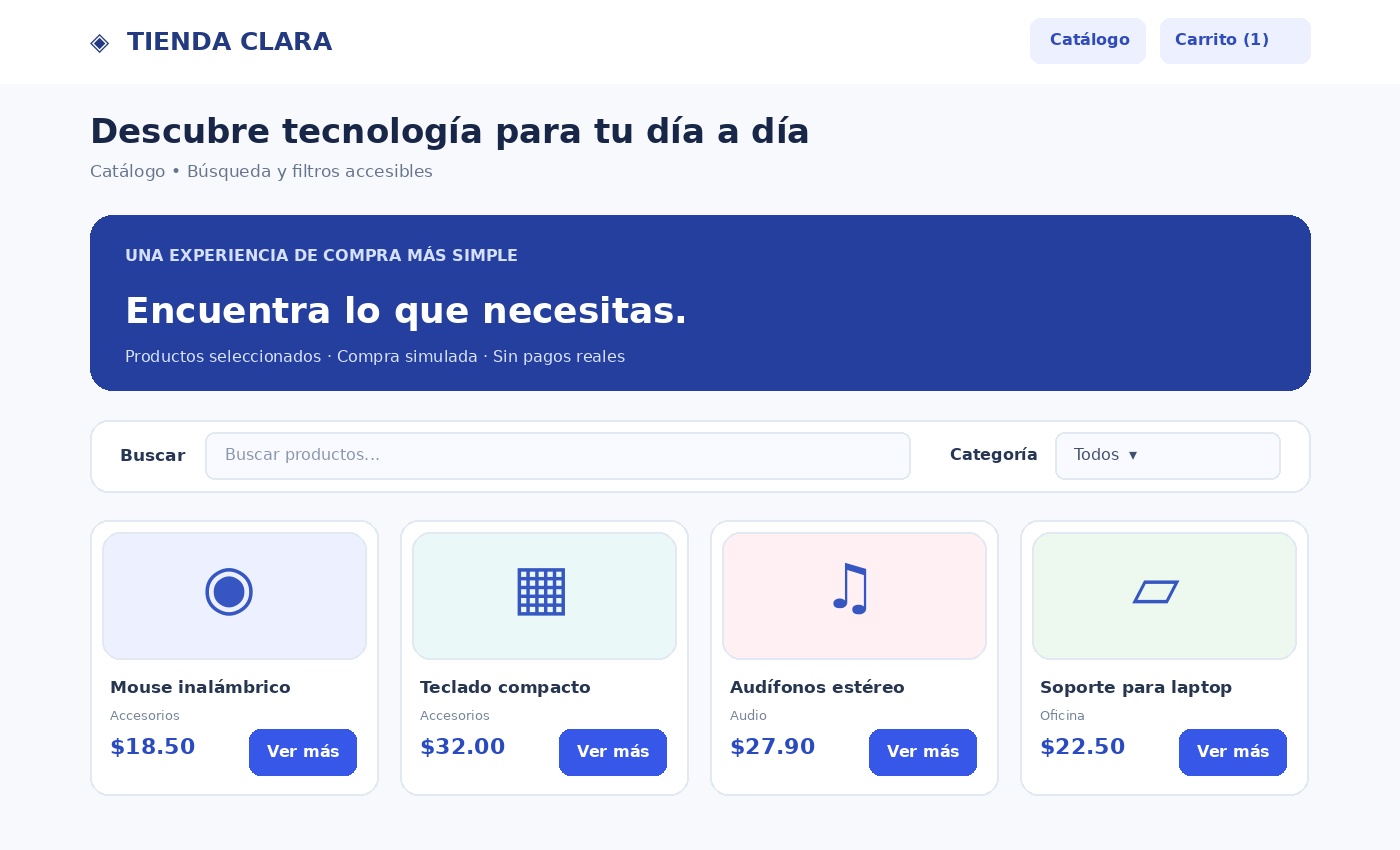
\includegraphics[width=0.85\textwidth]{imagenes/figura1_catalogo.png}
    \caption{Catálogo de productos y búsqueda en vivo (R1, T1).}
    \label{fig:catalogo}
\end{figure}
\textit{Explicación:} La Figura \ref{fig:catalogo} presenta la disposición del catálogo de productos con búsqueda en tiempo real e insignia de compra simulada, permitiendo al usuario comprobar R1 y completar T1.

\begin{figure}[H]
    \centering
    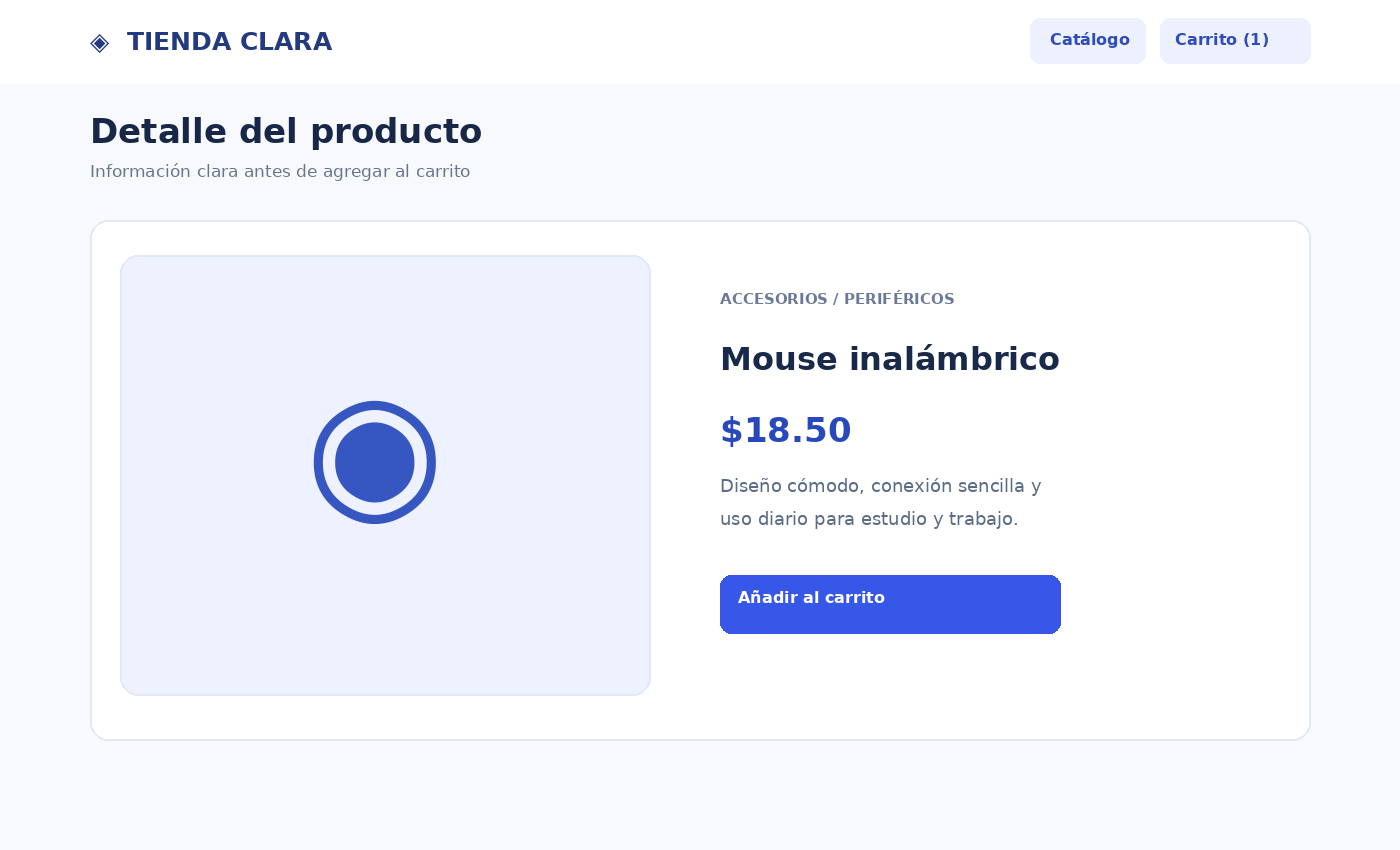
\includegraphics[width=0.85\textwidth]{imagenes/figura2_detalle.png}
    \caption{Vista de detalle y características del producto (R2, T1).}
    \label{fig:detalle}
\end{figure}
\textit{Explicación:} La Figura \ref{fig:detalle} organiza la descripción, precio unitario y llamado a la acción primario para apoyar una selección informada, dando cumplimiento a R2.

\begin{figure}[H]
    \centering
    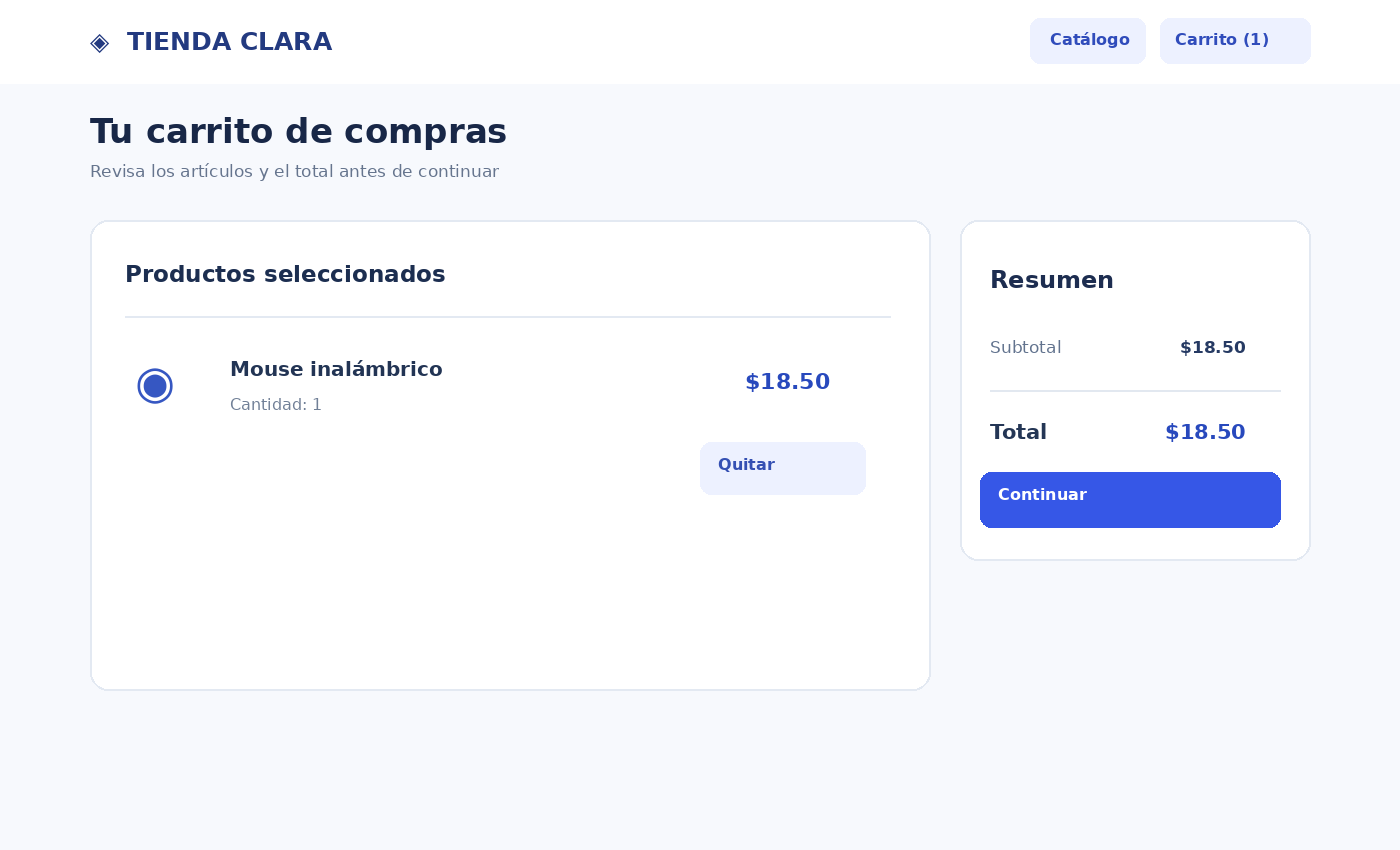
\includegraphics[width=0.85\textwidth]{imagenes/figura3_carrito.png}
    \caption{Gestión interactiva del carrito de compras (R3, T2).}
    \label{fig:carrito}
\end{figure}
\textit{Explicación:} La Figura \ref{fig:carrito} exhibe el desglose de artículos agregados, cálculo dinámico de subtotales y opciones de modificación, respaldando el requisito R3 y la tarea T2.

\begin{figure}[H]
    \centering
    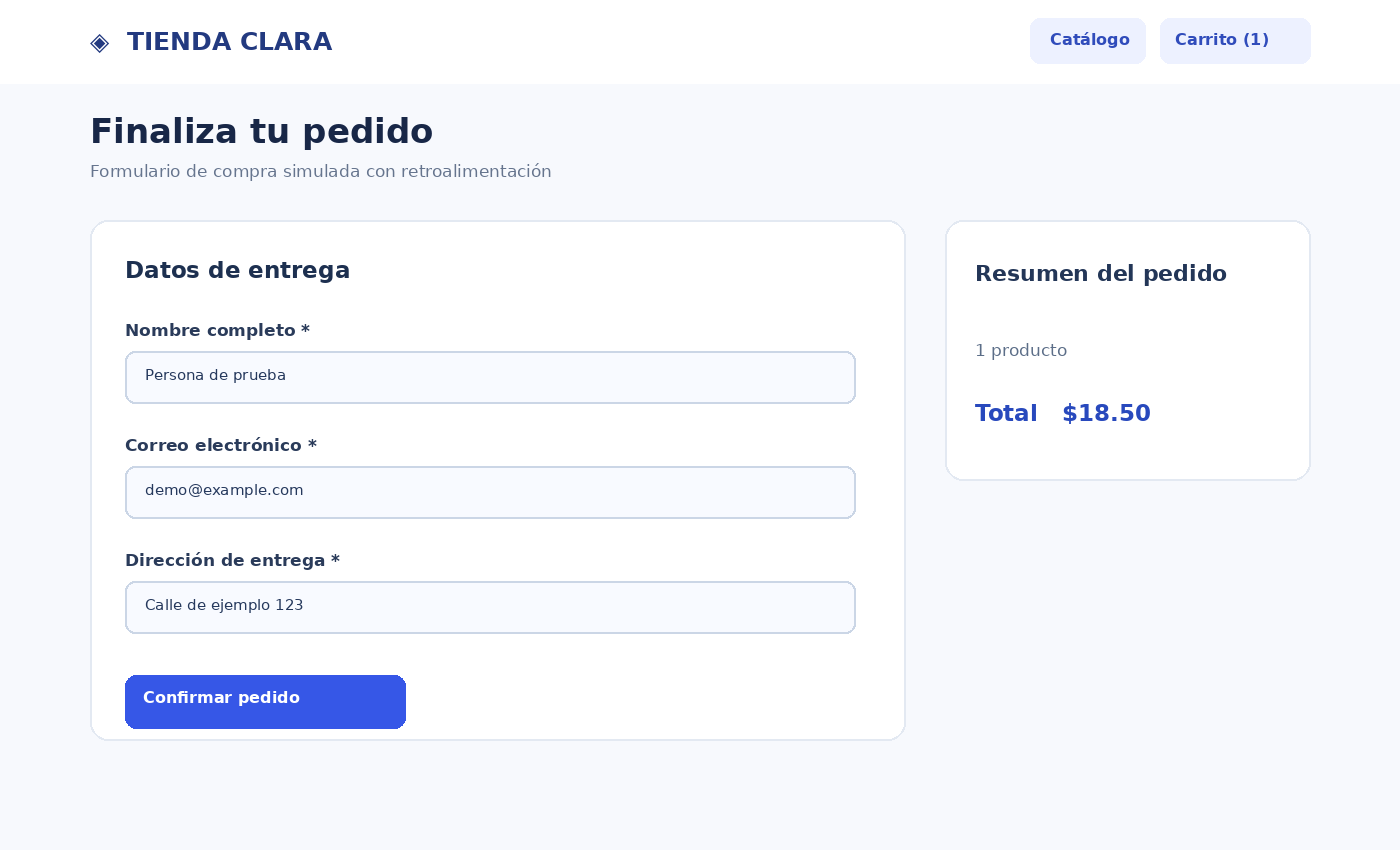
\includegraphics[width=0.85\textwidth]{imagenes/figura4_formulario.png}
    \caption{Formulario de checkout y resumen de orden (R4, T3).}
    \label{fig:formulario}
\end{figure}
\textit{Explicación:} La Figura \ref{fig:formulario} agrupa los campos de envío junto al resumen monetario para minimizar la carga cognitiva del comprador (R4 y T3).

\begin{figure}[H]
    \centering
    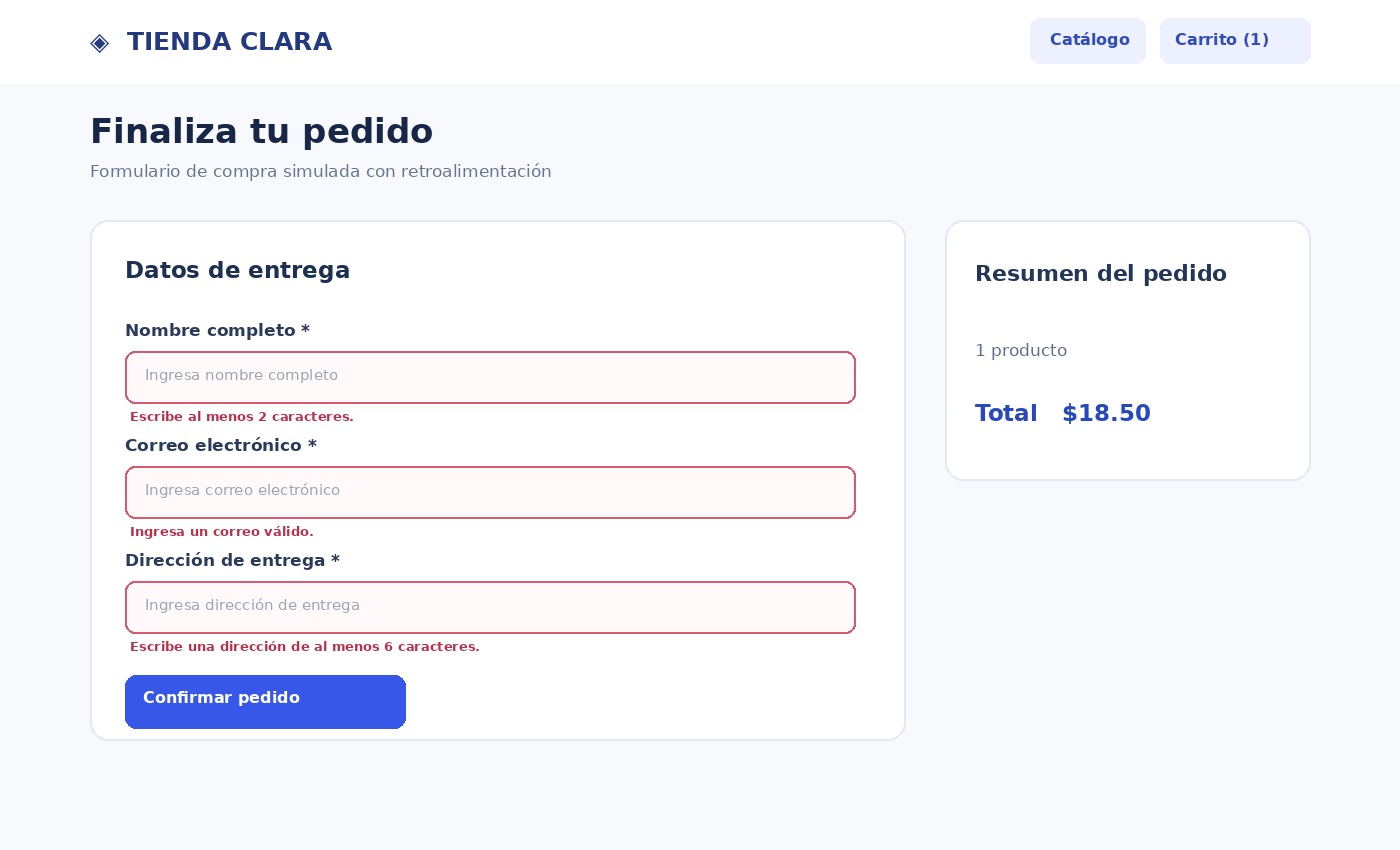
\includegraphics[width=0.85\textwidth]{imagenes/figura5_validaciones.png}
    \caption{Validación contextual y recuperación de errores (R5, T3).}
    \label{fig:validaciones}
\end{figure}
\textit{Explicación:} La Figura \ref{fig:validaciones} ilustra los avisos de error ubicados junto a los campos involucrados, preservando los datos ya completados y facilitando la corrección (R5).

\begin{figure}[H]
    \centering
    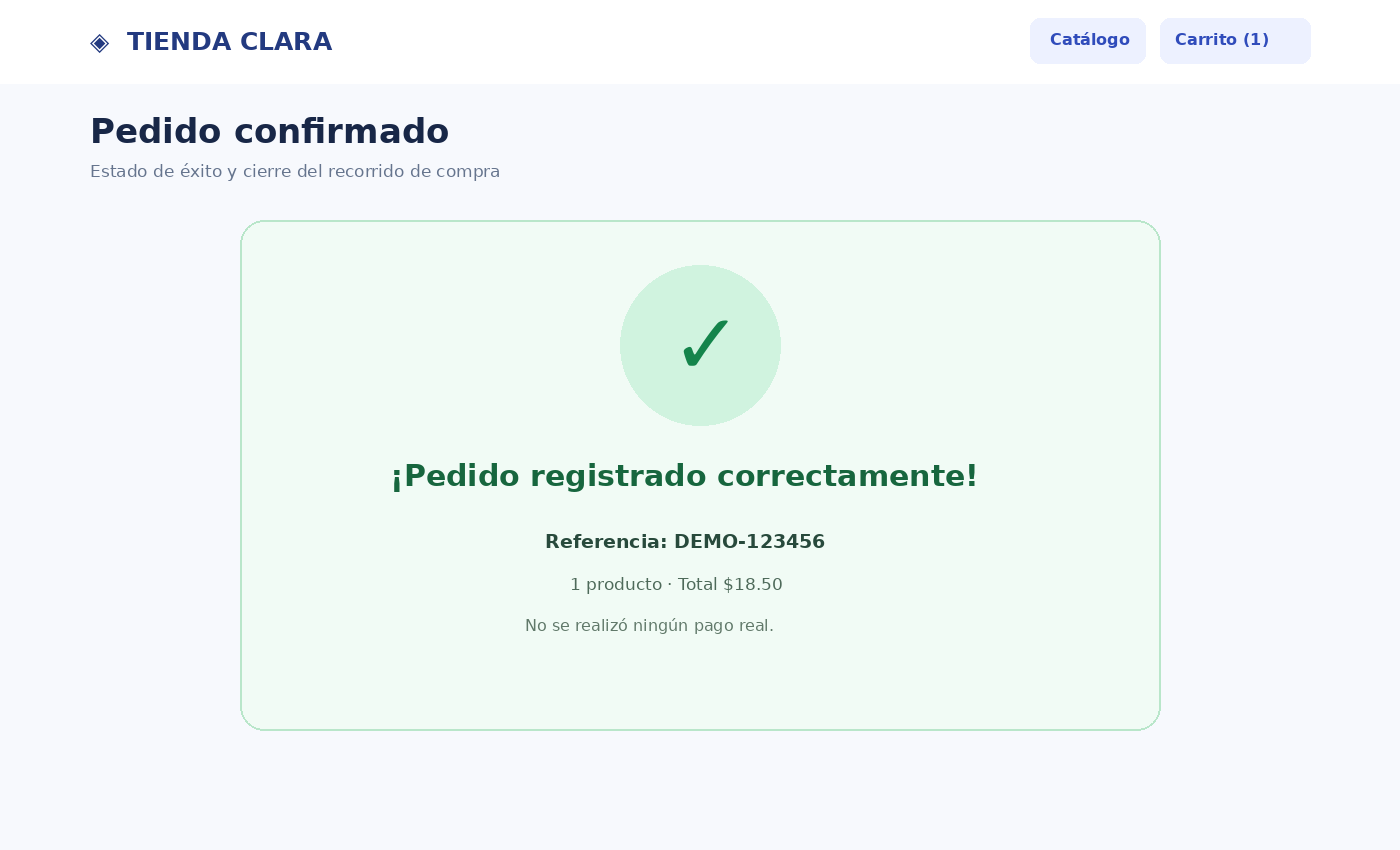
\includegraphics[width=0.85\textwidth]{imagenes/figura6_confirmacion.png}
    \caption{Pantalla de confirmación con identificador de pedido (R6, T3).}
    \label{fig:confirmacion}
\end{figure}
\textit{Explicación:} La Figura \ref{fig:confirmacion} comunica inequívocamente el éxito de la simulación, otorgando una referencia visible única (\texttt{DEMO-XXXXXX}) para R6.

\subsubsection{Evidencia de Colaboración Grupal en GitHub}
Se implementó un flujo riguroso de control de versiones en GitHub con cuatro ramas especializadas, cuatro Issues técnicos y sus correspondientes Pull Requests (Tabla \ref{tab:github_colaboracion}).

\begin{table}[H]
\centering
\caption{Matriz de contribuciones individuales, ramas, Issues y Pull Requests en GitHub.}
\label{tab:github_colaboracion}
\vspace{0.2cm}
\begin{tabularx}{\textwidth}{l c c c X}
\toprule
\textbf{Integrante} & \textbf{Rama Git} & \textbf{Issue} & \textbf{PR} & \textbf{Aporte Específico} \\
\midrule
Sebastián Vaca & \texttt{sebastian} & \#1 & \#5 & Estructuración del informe inicial, marco de objetivos y matriz de diagnóstico. \\
Andrew Lara & \texttt{andrew} & \#2 & \#6 & Desarrollo funcional del prototipo base v1 y estabilización técnica. \\
Verónica Jaque & \texttt{veronica} & \#3 & \#7 & Rediseño de interfaz v2, micro-interacciones, toast dinámico y accesibilidad. \\
Elizabeth De la Cruz & \texttt{elizabeth} & \#4 & \#8 & Protocolo empírico de pruebas, auditoría WCAG, conversión PDF y consolidación. \\
\bottomrule
\end{tabularx}
\end{table}

\subsection{Habilidades blandas empleadas en la tarea}
Durante la ejecución colaborativa de la práctica se ejercitaron activamente las siguientes competencias:
\begin{itemize}
    \item[$\blacksquare$] Liderazgo: Coordinación distribuida de tareas por componentes en Git.
    \item[$\blacksquare$] Trabajo en equipo: Sincronización continua de ramas y revisión cruzada de código.
    \item[$\blacksquare$] Comunicación asertiva: Alineación conceptual sobre los requerimientos de usabilidad.
    \item[$\blacksquare$] La empatía: Modelado centrado en las necesidades reales del usuario final.
    \item[$\blacksquare$] Pensamiento crítico: Diagnóstico analítico de fricciones en el recorrido de compra.
    \item[$\blacksquare$] Flexibilidad: Iteración del prototipo desde v1 hacia v2 según observaciones.
    \item[$\blacksquare$] La resolución de conflictos: Consenso en decisiones técnicas de arquitectura.
    \item[$\blacksquare$] Adaptabilidad: Manejo de múltiples herramientas (HTML/CSS/JS, LaTeX, Git).
    \item[$\blacksquare$] Responsabilidad: Cumplimiento riguroso de los plazos y entregables académicos.
\end{itemize}

\subsection{Conclusiones}
\begin{enumerate}
    \item La aplicación de metodologías de diseño centrado en el usuario permitió transformar una experiencia tradicional de compra en una interfaz estructurada, intuitiva y accesible, confirmando que la clarificación del flujo reduce sustancialmente la incertidumbre operativa del comprador.
    \item La evaluación empírica con participantes reales validó cuantitativamente la superioridad de la versión final (v2), alcanzando una reducción superior al 38\% en los tiempos de respuesta y eliminando por completo los bloqueos por errores de formulario gracias a las validaciones contextuales con foco guiado.
    \item La incorporación de pautas WCAG 2.1 (Nivel AA) como enlaces skip-link, ratios de contraste superiores a 9:1 y anuncios dinámicos vía \texttt{aria-live="polite"} demostró que la accesibilidad no compromete la estética moderna de una interfaz, sino que potencia transversalmente la experiencia de uso para todo tipo de usuarios.
\end{enumerate}

\subsection{Recomendaciones}
\begin{enumerate}
    \item Para futuras iteraciones del prototipo académico, se recomienda implementar un historial de órdenes anteriores almacenado de forma segura en almacenamiento del cliente para facilitar compras recurrentes.
    \item Integrar filtrado multifacético que combine rangos de precios personalizables con búsqueda fonética para mitigar fallas tipográficas del usuario.
    \item Extender las pruebas de usabilidad a usuarios con discapacidad visual empleando lectores de pantalla especializados para auditar la cadencia y claridad de las descripciones contextuales.
\end{enumerate}

\subsection{Referencias}
\vspace{-3em}
\renewcommand{\refname}{}
\bibliographystyle{ieeetr}
\bibliography{sample}

\nocite{nielsen1994heuristics}
\nocite{w3c2023wcag}
\nocite{juano2026hci}
\nocite{davidpe2026grupo2}
\nocite{mauri2026grupo3}

\end{document}
